% J12: one classifier per constraint sorts constraints into active / inactive / unpredictable
% Shared preamble for the graphical abstracts (homepage "Latest journal articles").
% Build: bash _tikz/papers/build.sh  (writes images/papers/Jxx.svg)
% Classic TikZ look: white background, black text and arrows, standard xcolor
% colors for the elements (independent of the website theme).
\documentclass[tikz,border=0pt]{standalone}
\usepackage[T1]{fontenc}
\usepackage{textcomp}
\usepackage[scaled=0.95]{helvet}
\renewcommand\familydefault{\sfdefault}
\usetikzlibrary{arrows.meta,calc,positioning,patterns,decorations.pathreplacing}
% ---- classic colors (xcolor names) ----
\colorlet{main}{blue!70!black}   % primary elements
\colorlet{lite}{blue!35}         % connections
\colorlet{pale}{blue!8}          % light fills
\colorlet{acc}{red!75!black}     % highlights / outputs
\colorlet{good}{green!55!black}  % storage, positive
\colorlet{warn}{orange!85!black} % uncertain
\colorlet{sun}{orange}
\colorlet{rule}{black!35}
\colorlet{ink}{black}
\colorlet{muted}{black!60}
\colorlet{bg}{white}
\tikzset{
  every picture/.style={line cap=round, line join=round},
  head/.style={font=\fontsize{8.5}{10}\selectfont\bfseries, text=ink},
  sub/.style={font=\fontsize{6.6}{8}\selectfont, text=muted},
  lab/.style={font=\fontsize{7.2}{8.6}\selectfont, text=ink},
  flow/.style={-{Stealth[length=2.2mm,width=2mm]}, draw=black, line width=0.9pt},
  card/.style={draw=black!60, line width=0.6pt, fill=white, rounded corners=1mm},
  banner/.style={draw=black, line width=0.6pt, fill=black!4, text=black,
                 font=\fontsize{7.4}{9}\selectfont\bfseries\boldmath, inner sep=1.6mm},
}
% canvas 8 x 6 cm (4:3), white
\newcommand\canvas{\fill[bg] (0,0) rectangle (8,6);}

\begin{document}
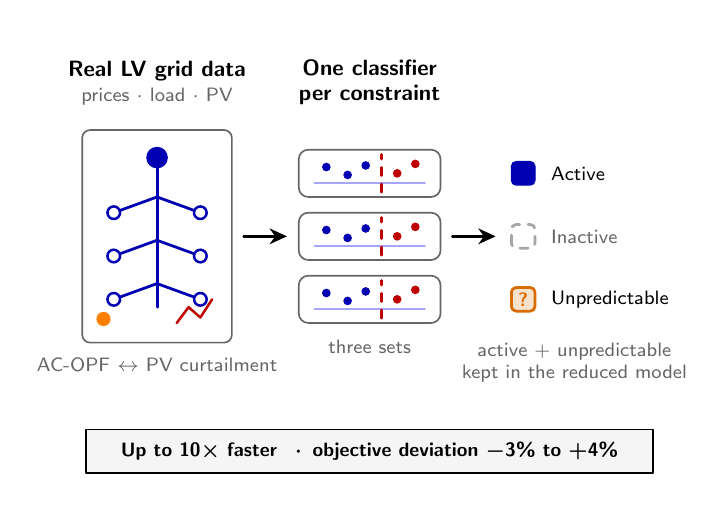
\begin{tikzpicture}
\canvas
% 1. real LV grid data
\node[head] at (1.3,5.45) {Real LV grid data};
\node[sub]  at (1.3,5.12) {prices $\cdot$ load $\cdot$ PV};
\draw[card] (0.35,2.0) rectangle (2.25,4.7);
% feeder: transformer + radial buses
\filldraw[fill=main, draw=main] (1.3,4.35) circle (0.13);
\draw[main, line width=1.1pt] (1.3,4.22) -- (1.3,2.45);
\foreach \y in {3.85,3.3,2.75} {
  \draw[main, line width=1pt] (1.3,\y) -- (0.75,\y-0.2) (1.3,\y) -- (1.85,\y-0.2);
  \filldraw[fill=white, draw=main, line width=0.9pt] (0.75,\y-0.2) circle (0.08);
  \filldraw[fill=white, draw=main, line width=0.9pt] (1.85,\y-0.2) circle (0.08);}
% small PV + price sparkline
\fill[sun] (0.62,2.3) circle (0.09);
\draw[acc, line width=0.9pt] (1.55,2.25) -- (1.7,2.45) -- (1.85,2.32) -- (2.0,2.55);
\node[sub] at (1.3,1.72) {AC-OPF $\leftrightarrow$ PV curtailment};
\draw[flow] (2.4,3.35) -- (2.95,3.35);
% 2. one classifier per constraint
\node[head, align=center] at (4.0,5.3) {One classifier\\[-1pt]per constraint};
\foreach \y in {4.15,3.35,2.55} {
  \draw[card, rounded corners=1.2mm] (3.1,\y-0.3) rectangle (4.9,\y+0.3);
  \draw[lite, line width=0.8pt] (3.3,\y-0.12) -- (4.7,\y-0.12);
  \foreach \x/\d/\c in {3.45/0.08/main,3.72/-0.02/main,3.95/0.1/main,4.35/0.0/acc,4.58/0.12/acc} \fill[\c] (\x,\y+\d) circle (0.055);
  \draw[acc, line width=0.9pt, dashed] (4.15,\y-0.24) -- (4.15,\y+0.24);}
\node[sub] at (4.0,1.95) {three sets};
\draw[flow] (5.05,3.35) -- (5.6,3.35);
% 3. three sets
\filldraw[fill=main, draw=main, rounded corners=0.6mm] (5.8,4.0) rectangle ++(0.3,0.3);
\draw[rule, line width=1pt, dashed, rounded corners=0.6mm] (5.8,3.2) rectangle ++(0.3,0.3);
\filldraw[fill=warn!20, draw=warn, line width=1pt, rounded corners=0.6mm] (5.8,2.4) rectangle ++(0.3,0.3);
\node[font=\fontsize{7}{7}\selectfont\bfseries, text=warn] at (5.95,2.55) {?};
\node[lab, anchor=west] at (6.18,4.15) {Active};
\node[sub, anchor=west] at (6.18,3.35) {Inactive};
\node[lab, anchor=west] at (6.18,2.55) {Unpredictable};
\node[sub, align=center] at (6.6,1.75) {active + unpredictable\\kept in the reduced model};
% result
\node[banner, minimum width=7.2cm] at (4,0.62)
   {Up to 10$\times$ faster \enspace$\cdot$\enspace objective deviation $-$3\% to $+$4\%};
\end{tikzpicture}
\end{document}
